\documentclass[11pt, handout]{beamer}
\usetheme{Boadilla}

\usepackage[utf8]{inputenc}
\usepackage{amsmath}
\usepackage{amsfonts}
\usepackage{amssymb}
\usepackage[dvipsnames]{xcolor}
\usepackage{tikz}
\usepackage{setspace}

\usetikzlibrary{positioning, arrows.meta}

\title{Lab 6: Little More on  Instrumental Variables}
\subtitle{Causal Inference}
\author{Chanhyuk Park and Xiangyu Song}
\date{}
\institute{Washington University in St. Louis}

\begin{document}

\begin{frame}
    \titlepage
\end{frame}

\begin{frame}{OLS Fails}
    \begin{itemize}[<+->]
        \item Consider the structural model: $Y_i = \alpha + \tau D_i + \epsilon_i$
        \vspace{0.8em}
        \item With observational data, we rarely have random assignment of $D$
        \vspace{0.8em}
        \item \textit{Endogeneity} occurs when $Cov(\epsilon_i, D_{i}) \neq 0$ e.g. \textcolor{blue}{omitted variable bias}
        \vspace{0.8em}
        \item The OLS estimator $\hat{\tau}_{OLS}$ converges to:
        \begin{equation*}
            \begin{aligned}
                \frac{Cov(Y_{i}, D_i)}{Var(D_i)} \pause &= \frac{Cov(\tau D_{i} + \epsilon_i, D_{i})}{Var(D_{i})} \\ \pause
                 &= \tau + \frac{Cov(\epsilon_i, D_i)}{Var(D_i)} \\
            \end{aligned}
        \end{equation*}
        \vspace{0.8em}
        \item We are attributing the effect of the error term to the treatment.
    \end{itemize}
\end{frame}

\begin{frame}{The IV Solution: The DAG}
    \begin{itemize}
        \item A solution: instrumental variable $Z$
    \end{itemize}
    \vspace{0.8em}
    \begin{center}
        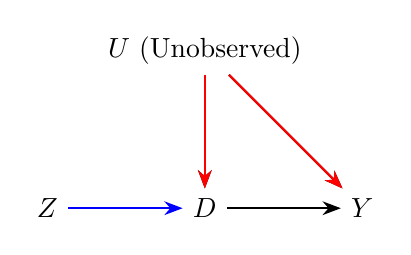
\begin{tikzpicture}[node distance=2cm, >=Stealth, thick]
            \node (Z) {$Z$};
            \node (D) [right of=Z] {$D$};
            \node (Y) [right of=D] {$Y$};
            \node (U) [above of=D] {$U$ (Unobserved)};
            
            \draw[->, blue] (Z) -- (D);
            \draw[->] (D) -- (Y);
            \draw[->] (U) -- (D);
            \draw[->] (U) -- (Y);
            \only<2->{
                \draw[->, red] (U) -- (D);
                \draw[->, red] (U) -- (Y);
            }
        \end{tikzpicture}
    \end{center}
    \vspace{0.8em}
    \begin{itemize}[<+->]
        \item \textit{The Relevance Condition:} There is a \textcolor{blue}{strong arrow} from $Z$ to $D$.
        \vspace{0.8em}
        \item \textit{The Exclusion Restriction:} There is \textcolor{red}{no direct arrow} from $Z$ to $Y$.
    \end{itemize}
\end{frame}

\begin{frame}{Core IV Assumptions}
    \begin{itemize}[<+->]
        \item \textit{Relevance:} $Z$ must be correlated with $D$. \\ If $Z$ does not capture $D$, then it is useless!
        \vspace{0.8em}
        \item \textit{Independence (Randomized Assignment):} \\ $Z$ should be independent from $Y$ and $D$ or as good as random.
        \begin{itemize}
            \item Formally: $Z \perp \{Y(d, z), D(z)\}$.
        \end{itemize}
        \vspace{0.8em}
        \item \textit{Exclusion Restriction:} $Z$ affects $Y$ \textit{only} through $D$.
        \begin{itemize}
            \item Mathematically: $Cov(Z, \epsilon) = 0$.
        \end{itemize}
        \vspace{0.8em}
        \item \textit{Monotonicity:} The instrument affects everyone in the same direction. 
        \begin{itemize}
            \item There are no \textcolor{red}{Defiers} (people who do the opposite of what $Z$ suggests).
            \item $D_i(1) \geq D_i(0)$ for all $i$.
        \end{itemize}
    \end{itemize}
\end{frame}

\begin{frame}{Are the Assumptions Testable?}
    \begin{itemize}[<+->]
        \item \textcolor{blue}{\textit{Relevance}} ($Cov(Z, D) \neq 0$): \textcolor{teal}{Yes, directly.}
        \begin{itemize}
            \item First Stage regression $D$ on $Z$
        \end{itemize}
        \vspace{0.8em}
        \item \textcolor{blue}{\textit{Independence}} ($Z \perp \{Y(d, z), D(z)\}$): \textcolor{orange}{Partially.}
        \begin{itemize}
            \item Like an RCT, we can perform \textit{balance tests}.
            \item If $Z$ is correlated with pre-treatment covariates (e.g., age, gender, baseline wealth), then $Z$ is likely not as-good-as-random.
        \end{itemize}
        \vspace{0.8em}
        \item \textcolor{blue}{\textit{Exclusion Restriction}} ($Z \perp \epsilon | D$): \textcolor{red}{No.}
        \begin{itemize}
            \item This is a \textit{fundamentally untestable} assumption
            \item It involves the \textit{unobserved error term}
        \end{itemize}
        \vspace{0.8em}
        \item \textcolor{blue}{\textit{Monotonicity}} (No Defiers): \textcolor{red}{No.}
        \begin{itemize}
            \item We never observe both $D_i(1)$ and $D_i(0)$
        \end{itemize}
    \end{itemize}
\end{frame}

\begin{frame}{The Taxonomy of Compliance}
    \begin{itemize}[<+->]
        \item Suppose binary instrument $Z$ and binary treatment $D(Z)$
        \vspace{0.8em}
        \item \textcolor{blue}{Compliers}: $D_i(1)=1, D_i(0)=0$ (They follow the instrument).
        \vspace{0.8em}
        \item \textcolor{darkgray}{Always-takers}: $D_i(1)=1, D_i(0)=1$ (They take $D$ regardless of $Z$).
        \vspace{0.8em}
        \item \textcolor{darkgray}{Never-takers}: $D_i(1)=0, D_i(0)=0$ (They avoid $D$ regardless of $Z$).
        \vspace{0.8em}
        \item \textcolor{red}{Defiers}: $D_i(1)=0, D_i(0)=1$ (We assume these do not exist; Monotonicity).
        \vspace{0.8em}
        \item \textit{Crucial Point:} \\ Never observe which group an individual belongs to (just like the fundamental problem of causal inference). \\ Compliance is a \textit{latent} characteristic.
    \end{itemize}
\end{frame}

\begin{frame}{ITT Decomposition}
    \begin{itemize}[<+->]
        \item The \textit{Intent-to-Treat (ITT)} is the effect of $Z$ on $Y$: $E[Y_i | Z_i=1] - E[Y_i | Z_i=0]$.
        \vspace{0.8em}
        \item We can decompose this using the Law of Total Probability:
        \begin{equation*}
            \begin{aligned}
                ITT = &\pi_C \cdot E[Y_i(D_{i}(\textcolor{blue}{Z_{i} = 1}) = 1) - Y_i(D_{i}(\textcolor{blue}{Z_{i} = 0)} = 0) | C] + \\
                      &\pi_A \cdot E[Y_i(D_{i}(\textcolor{blue}{Z_{i} = 1}) = 1) - Y_i(D_{i}(\textcolor{blue}{Z_{i} = 0)} = 1) | A] + \\ 
                      &\pi_N \cdot E[Y_i(D_{i}(\textcolor{blue}{Z_{i} = 1}) = 0) - Y_i(D_{i}(\textcolor{blue}{Z_{i} = 0)} = 0) | N]
            \end{aligned}
        \end{equation*}
        \vspace{0.8em}
        \item \textit{Exclusion Restriction} + Taxonomy \\ $\implies$ zero effect on Always-takers and Never-takers
        \vspace{0.8em}
        \item The ITT simplifies to:
        \begin{equation*}
            ITT = \pi_C \cdot \text{\textit{Effect on Compliers}}
        \end{equation*}
        \item If treatment effect is homogeneous across these groups, $ITT = ATE$
    \end{itemize}
\end{frame}

\begin{frame}{From ITT to LATE}
    \begin{itemize}[<+->]
        \item The \textit{First Stage} is the effect of $Z$ on $D$: $E[D_i | Z_i=1] - E[D_i | Z_i=0]$.
        \vspace{0.8em}
        \item The IV Estimator (Wald) is the ratio:
        \begin{equation*}
            \beta_{IV} = \frac{E[Y|Z=1] - E[Y|Z=0]}{E[D|Z=1] - E[D|Z=0]} = \frac{\pi_C \cdot E[Y(1)-Y(0)|C]}{\pi_C}
        \end{equation*}
        \vspace{0.8em}
        \item $\beta_{IV} = E[Y_i(1) - Y_i(0) | \text{Compliers}]$
        \vspace{0.8em}
        \item This is the \textcolor{blue}{Local Average Treatment Effect (LATE)}.
    \end{itemize}
\end{frame}

\begin{frame}{LATE: Why the ``Local'' Matters}
    \begin{itemize}[<+->]
        \item The IV estimate is \textit{only} representative of the Compliers of the Instrument.
        \vspace{0.8em}
        \item \textcolor{Green}{Different instruments identify different effects}
        \vspace{0.8em}
        \item Example: The effect of \textit{Military Service} on \textit{Earnings}
        \begin{itemize}
            \item $Z_1$: The Draft Lottery (moves those who wouldn't volunteer but go if drafted).
            \item $Z_2$: Proximity to a recruitment center (moves those on the margin of volunteering).
        \end{itemize}
        \vspace{0.8em}
        \item $\beta_{Z_{2}}$(marginal volunteer) $>$ $\beta_{Z_{1}}$ (reluctant draftee)
        \vspace{0.8em}
        \item \textit{Takeaway:} \textcolor{red}{``Who are the compliers for this specific instrument?''}
    \end{itemize}
\end{frame}

\begin{frame}{Conclusion}
    \begin{itemize}[<+->]
        \item IV recovers the \textit{Average Treatment Effect (ATE)} if TE is homogeneous
        \vspace{0.8em}
        \item If effects are heterogeneous, IV gives us the \textit{LATE}
        \vspace{0.8em}
        \item Different IV $\implies$ Different LATE
        \vspace{0.8em}
        \item Assumptions!!!
            \begin{itemize}
                \item \textit{Exclusion Restriction} is a key
                \vspace{0.8em}
                \item \textit{Relevance} is the second key
                \vspace{0.8em} 
                \item \textit{Monotonicity} is the third key
            \end{itemize}
        \vspace{0.8em}
    \end{itemize}
\end{frame}
\end{document}
